\documentclass[12pt, utf8]{beamer}
\usepackage[ngerman]{babel}
\usepackage{xcolor}
\usepackage{graphicx}
\usepackage {listingsutf8}
\usepackage{multicol}

%AnnArbor | Antibes | Bergen |
% Berkeley | Berlin | Boadilla |
% boxes | CambridgeUS | Copenhagen |
% Darmstadt | default | Dresden |
% Frankfurt | Goettingen |Hannover |
% Ilmenau | JuanLesPins | Luebeck |
% Madrid | Malmoe | Marburg |
% Montpellier | PaloAlto | Pittsburgh |
% Rochester | Singapore | Szeged |
% Warsaw

%Einbinden des Themes
\usetheme{Berlin}
%Standard Angaben
\author{Lucius Bachmann, Fabio Sulzer, Frank Müller, Oliver Wisler}
\title{SwissDefcon}
\date{\today}


\definecolor{dkgreen}{rgb}{0,0.6,0}
\definecolor{gray}{rgb}{0.5,0.5,0.5}
\definecolor{mauve}{rgb}{0.58,0,0.82}


\begin{document}

\begin{frame}
\titlepage
\end{frame}

\begin{frame}[allowframebreaks,allowdisplaybreaks]
\frametitle{Inhaltsverzeichnis}
\setcounter{tocdepth}{1}
\tableofcontents
\end{frame}


\section{Einführung}
\subsection{Spielidee}
\begin{frame}{Spielidee}
\begin{itemize}
\item Verfeindete Kantone bekämpfen sich
\item Dabei stehen verschiedene Waffen und Gebäude zur Verfügung
\item Beschränkt durch das Kantonsbudget
\end{itemize}
\end{frame}

\section{Spielstatus}

\subsection{Spielstatus}
\begin{frame}{Spielstatus}
Was muss gespeichert werden?
\begin{multicols}{2}
\begin{itemize}
\item Spielerdaten
\begin{itemize}
\item Geld
\item Gebiet
\item Objekte
\end{itemize}
\item Objektdaten
\begin{itemize}
\item Standort
\item Lebenspunkte
\end{itemize}
\end{itemize}
\end{multicols}
\end{frame}

\subsection{Verwaltung Spielstatus}
\begin{frame}{Verwaltung}
	\begin{itemize}
		\item für jedes Spiel eine eigene Spielinstanz
			\begin{itemize}
		\item jede Instanz verwaltet die ihr zugehörigen Spieler
		\item verwaltet den Spielstand
			\end{itemize}
		\item mehrere Spiele $=$ mehrere Instanzen
	\end{itemize}
\end{frame}

\section{Spielregeln}
\subsection{Regeln}
\begin{frame}[allowframebreaks]
	\begin{itemize}
\item das Spiel ist rundenbasiert
\item Die Zeit pro Runde ist begrenzt
\item Während der Runde können Objekte platziert und bewegt werden
\item Die Anzahl Objekte ist durch das Kantonsbudget beschränkt
\item Nach dem Rundenende wird der Spielzug ausgeführt
\item Für die Zerstörung von Gebäuden und dezimierung der Bevölkerung gibt es Geld
\item Der Spieler der nach einer bestimmten Anzahl Runden am meisten Geld hat gewinnt
\item Spieler ohne Bevölkerung scheiden aus
\end{itemize}
	\begin{exampleblock}{Implementation}
		\begin{itemize}
\item jedes Spielobjekt beinhaltet seine Regeln
\item keine Regelklasse
\item Überprüfung durch den Server
\end{itemize}
\end{exampleblock}
\end{frame}


\subsection{Implementation}
\begin{frame}{Implementation}
\begin{figure}
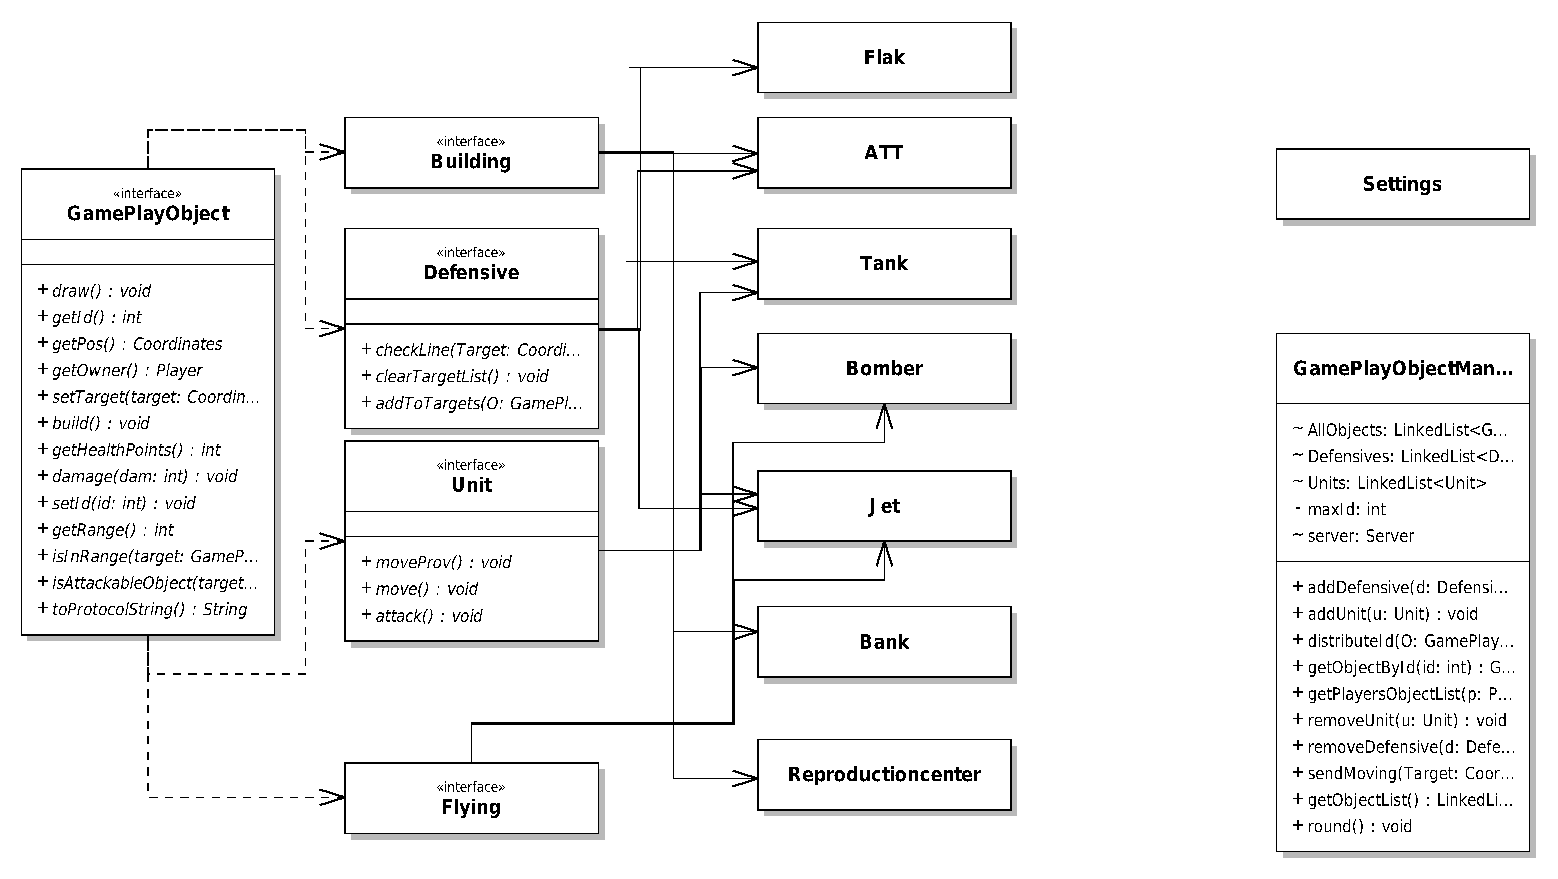
\includegraphics[width=9cm]{images/GamePlayObjects.ps}
\caption{Klassendiagramm der Spielobjekte}
\end{figure}
\end{frame}

 
\section{Kommunikation}
\subsection{Discovery-Service}
\begin{frame}
Innerhalb eines LAN Netzwerkes.
\begin{exampleblock}{Server Broadcast}
Der Server sendet über Multicast ein Alive. \\
Der Client kann so vorhandene Server finden.\
\end{exampleblock}
alternativ direkt mit IP verbinden.
\end{frame}

\subsection{Chat und Broadcast}
\begin{frame}
	\begin{itemize}
		\item Der Server hat eine Liste mit allen Clients.
		\item Nachrichten werden per default an die Gruppe des Clients versendet.
			\begin{itemize}
				\item Lobby
				\item Spiel
			\end{itemize}
		\item Privatchat mit /msg
	\end{itemize}
\end{frame}
\subsection{Netzwerkprotokoll}
\begin{frame}
	\begin{definition}
		Anfangsbuchstaben des Befehls definiert Befehlsgruppe
		\begin{itemize}
			\item Verbindung
			\item Lobby
			\item Game
			\item Discovery
			\item Chat
		\end{itemize}
	\end{definition}
	\begin{definition}
		Danach 4 Buchstaben die den genauen Befehl definieren
	\end{definition}
\end{frame}

\section{Arbeitsplan}
\subsection{Arbeitsplan}
\begin{frame}
\centering
\begin{figure}
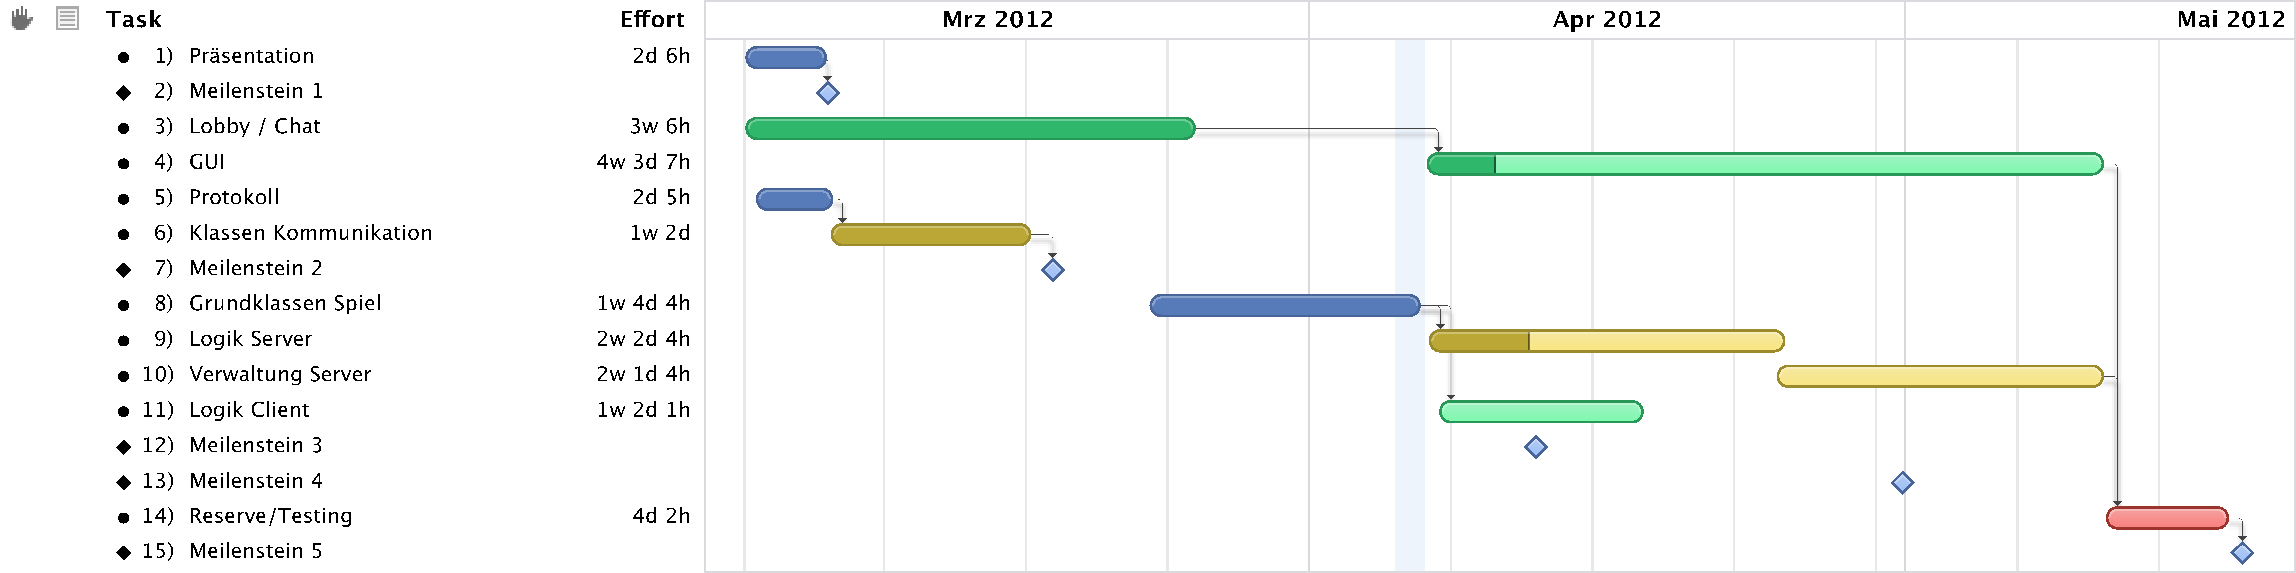
\includegraphics[width=11cm]{images/cs108.ps}
\caption{Arbeitsplan}
	\end{figure}
\end{frame}

\subsection{Ist} 
\begin{frame}{Ist-Stand}
\begin{itemize}
\item Lobby und Chat fertig
\item Serverstruktur fertig
\item bis jetzt geschrieben :
\begin{itemize}
\item 7939 Linien Code
\item 2050 Linien Kommentare
\end{itemize}

\end{itemize}
\end{frame}

\subsection{noch zu tun} 
\begin{frame}{to do}
\begin{itemize}
\item Ermittlung des Gewinners
\item Schnittstelle Clientparser $\leftrightarrow$ GUI des Spieles
\item Ausbau der GUI
\end{itemize}
\end{frame}

\section{Qualitätssicherung}
\subsection{Ist}
\begin{frame}{QS bis jetzt}
\begin{itemize}
\item eigene Log Klasse und viele Log-Messages
\item gute Dokumentation mit Javadoc
\item viele Kommentare (bis jetzt 20\%)
\item Aufteilung in Pakete nach Funktion
\item Servertests mit vielen Befehlen (ca. 3000 Befehle random)
\end{itemize}
\end{frame}

\subsection{noch geplant}
\begin{frame}
	\begin{exampleblock}{Unit Test}
		Bank
	\end{exampleblock}
\end{frame}


\section{Demo}
\subsection{Demo}
\begin{frame}{Demo}
\begin{itemize}
\item Discovery Service
\item Lobby
\item Chat und private Messaging
\item Spiel erstellen und starten
\item Server Broadcasts
\end{itemize}
\end{frame}

\end{document}
